% =============================================================================
% journal/paper/main.tex
%
% TODO: swap to mdpi.cls on template download.
%
% MDPI's LaTeX template (mdpi.cls + Definitions/ bundle) could not be
% retrieved: https://www.mdpi.com/authors/latex returns HTTP 403 (Cloudflare
% bot-protection) to both the fetch tool and a plain curl with a browser
% user-agent, on every guessed direct zip path. Third-party GitHub mirrors of
% mdpi.cls exist (e.g. github.com/ihrke/mdpi) but were NOT used here per the
% task's explicit instruction to fall back to the standard article class
% rather than substitute an unofficial copy of MDPI's class file.
%
% This file is written to be MDPI-structure-compatible so that swapping
% \documentclass{article} -> \documentclass[technologies]{mdpi} plus wrapping
% the front matter in MDPI's \Title/\Author/\Abstract/\Keywords macros should
% be a mechanical port once the real template is available. Until then this
% compiles standalone with pdflatex + bibtex.
% =============================================================================
\documentclass[11pt,a4paper]{article}

% --- Packages (kept minimal; swap for MDPI's Definitions/mdpi.cls list) ----
\usepackage[utf8]{inputenc}
\usepackage[T1]{fontenc}
\usepackage{amsmath,amssymb}
\usepackage{graphicx}
\usepackage{booktabs}
\usepackage[margin=2.5cm]{geometry}
\usepackage[colorlinks=true,citecolor=blue,linkcolor=blue,urlcolor=blue]{hyperref}
\usepackage[numbers,square,sort&compress]{natbib}
\usepackage{lineno}   % MDPI requires continuous line numbers on submission
\usepackage{xcolor}

% Inline TODO/pending markers, visible in the compiled PDF as a reviewing aid.
% Remove (or \renewcommand to no-op) once results land.
\newcommand{\todonote}[1]{\textcolor{red}{\textbf{[TODO: #1]}}}
\newcommand{\respending}[1]{\textcolor{red}{\textbf{[RESULTS-PENDING: #1]}}}

\linenumbers

% --- Front matter -----------------------------------------------------------
\title{\Large Machine Learning Methods for $n$-Colorant Printer Characterization: A Corrected and Extended Evaluation}

\author{
  Muhammad Hamza Zafar$^{1,*}$ \and Philip J. Green$^{1}$
}

\date{}

\begin{document}
\maketitle

\noindent
$^{1}$ Norwegian Colour and Visual Computing Laboratory, Department of Computer Science,
Norwegian University of Science and Technology (NTNU), Gjøvik, Norway\\
$^{*}$ Correspondence: muhammad.h.zafar@ntnu.no

% TODO: MDPI front matter also requires — Received/Revised/Accepted/Published
% dates (set by the journal on submission), Academic Editor, Citation block,
% and the special-issue field:
%   Journal: Technologies (MDPI)
%   Special Issue: "AI-Driven Color Models for Imaging, Formulation,
%     Appearance Measurement and Computer Vision"
%   Guest Editors: Eric J.J. Kirchner, Stephen Westland
%   Submission deadline: 30 August 2026

\begin{abstract}
\noindent
\todonote{Abstract stub -- fill in once Results/Discussion are drafted (Task 2).
MDPI Technologies caps the abstract at 200 words; single paragraph, no
citations, no undefined abbreviations.}
Printer color characterization maps a device's colorant inputs (CMY, CMYK, or
higher-channel combinations) to device-independent color coordinates (CIE
XYZ/Lab). A prior conference study (AIC 2025) compared 14 machine learning
methods against third-order polynomial regression for $n=3$ (CMY) inputs
across three printer datasets, finding no consistent advantage for the
learned models. That analysis is superseded here: its CIEDE2000 errors were
computed on normalized rather than physical XYZ values, understating errors
by roughly a factor of five. This paper reports corrected $n=3$ results,
extends the comparison to $n=4$ (CMYK) inputs, \respending{n$>$4 (CMYKOGV)
results, if the dataset lands in time}, and \respending{cross-printer /
newsprint generalization and direct-$\Delta E_{00}$-loss results, if those
experiments land in time}. \todonote{One-sentence headline finding once
available.}
\end{abstract}

\textbf{Keywords:} printer characterization; color management; CIEDE2000;
machine learning; Gaussian process regression; polynomial regression;
CMYK; $n$-colorant printing; ICC profiling

% =============================================================================
\section{Introduction}
% =============================================================================
\todonote{Extend the AIC 2025 introduction (Task 2, per docs/plans/07-paper.md).
Planned additions: (i) the lookup-table-inefficiency motivation for
higher-channel printing (Phil, Apr 2026 meeting) -- LUTs scale combinatorially
with the number of colorants, so device characterization methods that avoid
dense LUT construction become increasingly attractive as $n$ grows beyond 4;
(ii) restate Phil Green's two core questions verbatim: (a) can ML/AI match or
beat existing methods for $n \leq 4$ colorants, avoiding the need for
gray-component-replacement-style algorithms; (b) can AI handle $n>4$ colorant
systems (e.g. CMYKOGV) where classical polynomial methods are not designed to
scale; (iii) state explicitly that this paper corrects and supersedes the AIC
2025 conference numbers (forward-reference to the Methods correction
paragraph).}

% =============================================================================
\section{Related Work}
% =============================================================================
\todonote{Task 2. Prior device-characterization literature already in
refs.bib (Bala 2003; Cheung et al. 2004; Kang \& Anderson 1992; Tominaga
1993) plus the per-method ML references (Breiman 1984/2001; Cortes \& Vapnik
1995; Cover \& Hart 1967; Friedman 2001; Geladi \& Kowalski 1986; Hoerl \&
Kennard 1970; Rasmussen \& Williams 2006; Tibshirani 1996; Zou \& Hastie
2005). Add: Kiran's Optics Express $n$-colour paper and the PhD-work
benchmark Phil pointed to (both currently commented placeholders in
refs.bib -- exact citations pending); ISO/TC 130 standardization context
(Pang 2024); the FOGRA51 characterization dataset (Fogra 2020); the
colour-science library used throughout this pipeline (placeholder in
refs.bib, pending exact version/DOI).}

% =============================================================================
\section{Methods}
% =============================================================================

\subsection{Datasets}
\label{sec:datasets}

Three printer characterization datasets are used, each measured at 1{,}617
CMYK combinations under a shared measurement protocol (spectrophotometric
CIE Lab and CIE XYZ, D50 illuminant, 2\textdegree{} standard observer). Each
dataset is evaluated twice: once restricted to the $K=0$ subset with only
C, M, Y as inputs (818 rows -- the $n=3$ / CMY condition), and once using
the full sample set with C, M, Y, K as four inputs (1{,}617 rows -- the
$n=4$ / CMYK condition). Unlike the AIC 2025 conference version, the K
channel is never dropped while its rows are kept: doing so maps identical
CMY inputs to different XYZ outputs whenever K differs, which is an internal
label inconsistency, not a modeling choice.

\begin{table}[h]
\centering
\caption{Datasets used in the $n=3$ and $n=4$ conditions. Row counts are
pooled across all 5 cross-validation folds (Section~\ref{sec:protocol}), so
every sample is predicted exactly once.}
\label{tab:datasets}
\begin{tabular}{@{}llccc@{}}
\toprule
Dataset & Substrate & Inputs ($n$) & Rows & Source \\
\midrule
PC10  & Cardboard          & CMY  & 818  & APTEC PC10 (2023) \\
PC10  & Cardboard          & CMYK & 1{,}617 & APTEC PC10 (2023) \\
PC11  & Coated paper (CCNB)& CMY  & 818  & APTEC PC11 (2023) \\
PC11  & Coated paper (CCNB)& CMYK & 1{,}617 & APTEC PC11 (2023) \\
FOGRA51 & Reference (ISO 12647-2) & CMY & 818 & Fogra Research Institute \citep{fogra2020} \\
FOGRA51 & Reference (ISO 12647-2) & CMYK & 1{,}617 & Fogra Research Institute \citep{fogra2020} \\
\bottomrule
\end{tabular}
\end{table}

\todonote{Task 2/06: append IFRA newsprint (white-backing / black-backing, 43
press runs, 1{,}485 samples each, 36-band spectral $\rightarrow$ XYZ via
colour-science) once plan 03 lands, keeping wb and bb as separate rows per
Phil's instruction. Append CMYKOGV ($n=7$) row if that dataset arrives from
Phil/Will in time (plan 06).}

\subsection{Models}
\label{sec:models}

Fourteen regression methods are compared, matching the AIC 2025 study's
model set with two configuration corrections noted below. All models are
implemented input-dimension-agnostically, so the same code path serves the
$n=3$, $n=4$, and (if it lands) $n=7$ conditions.

\begin{table}[h]
\centering
\caption{Model registry (14 methods). Configurations match the AIC 2025
paper's best configs except where marked (*), which were degenerate there
(Lasso/Elastic Net at $\alpha=1.0$ collapsed to a constant predictor; SVR at
$\varepsilon=0.1$ produced an insensitivity tube covering 10\% of the target
range) and are replaced with standard, non-degenerate values.}
\label{tab:models}
\begin{tabular}{@{}ll@{}}
\toprule
Model & Configuration \\
\midrule
Polynomial regression (degree 3) & Full 3rd-order feature expansion + ordinary least squares \\
Ridge regression & $\alpha = 0.5$ \\
Lasso regression* & $\alpha = 10^{-3}$ \\
Elastic Net* & $\alpha = 10^{-3}$, $\ell_1$ ratio $= 0.5$ \\
Principal component regression & All components retained + Ridge ($\alpha=0.5$) \\
Partial least squares regression & 3 components \\
$k$-nearest neighbors & $k=5$, uniform weights \\
Support vector regression* & RBF kernel, $C=10$, $\gamma=$ scale, $\varepsilon = 0.01$ \\
Decision tree & Unconstrained depth \\
Random forest & 200 trees, max depth 15 \\
Gradient boosting & 200 estimators, learning rate 0.05, max depth 5 \\
Gaussian process regression & $\mathrm{Const} \times \mathrm{RBF} + \mathrm{WhiteKernel}(10^{-5})$, $y$-normalized \\
MLP (shallow) & 1 hidden layer, 64 units, L-BFGS \\
MLP (deep) & 3 hidden layers, 64 units each, L-BFGS \\
\bottomrule
\end{tabular}
\end{table}

\todonote{Task 2: add explicit equations for each model, in particular the
corrected 3rd-order polynomial expansion (Phil flagged an "odd expression" in
the AIC version's equation to fix). Every stochastic model above is seeded
(fixed seed = 42) for reproducibility, per CLAUDE.md's pinned-dependency
rule.}

\subsection{Evaluation Protocol}
\label{sec:protocol}

Each (dataset, model) pair is evaluated with 5-fold cross-validation
(fixed seed = 42). Folds are grouped by distinct input recipe (rounded to
6 decimal places) so that duplicate rows sharing the same colorant input
always fall in the same fold, preventing train/test leakage through
repeated measurements. Within each fold:

\begin{enumerate}
\item A \texttt{MinMax} scaler is fit on the training fold's inputs and,
  separately, on the training fold's XYZ targets -- scaling parameters are
  never estimated from the held-out fold.
\item The model is fit in the normalized (0--1) input/output space.
\item Predictions are generated in normalized space, then inverse-transformed
  back to physical XYZ using the training fold's target scaler.
\item Predicted XYZ values are clipped at zero (tristimulus values cannot
  be negative).
\item Both predicted and ground-truth XYZ are converted to CIE Lab under the
  D50 illuminant and 2\textdegree{} standard observer, and the per-sample
  color difference is computed with the CIE 2000 formula
  \citep{sharma2005ciede2000} via the \texttt{colour-science} library.
\end{enumerate}

Every sample in a dataset is held out exactly once across the 5 folds, so
the reported statistics pool over the entire dataset rather than a single
train/test split. Per repository convention (see CLAUDE.md), summary
statistics are the \textbf{median}, \textbf{95th percentile}, and
\textbf{maximum} of the per-sample $\Delta E_{00}$ distribution -- not the
mean or standard deviation, since color-difference errors are not normally
distributed and a small number of large outliers otherwise dominate a
mean-based summary.

As a data-integrity check, every dataset's own measured XYZ is round-tripped
through the same D50/2\textdegree{}/CIE-2000 conversion and compared against
its own measured Lab before any model is fit; a median absolute Lab
discrepancy above 0.6 aborts the run. This tripwire is a direct response to
the scale error described below, and guards against future recurrences (e.g.
accidentally feeding normalized XYZ into the Lab conversion).

\paragraph{Correction to the AIC 2025 conference results.}
The AIC 2025 conference version of this analysis computed $\Delta E_{00}$ on
normalized (0--1 scaled) XYZ values rather than on the physical 0--100 XYZ
scale, which understated the reported color differences by approximately a
factor of five. All results reported in this paper are corrected and
supersede the conference figures.

% =============================================================================
\section{Results}
% =============================================================================

\subsection{$n=3$ (CMY) -- Corrected}

Table~\ref{tab:n3} reports median, 95th-percentile, and maximum
$\Delta E_{00}$ for all fourteen models on the three $n=3$ (CMY) datasets,
pooled across the 5 cross-validation folds so that every one of the 818
$K=0$ samples per dataset is predicted exactly once. Figure~\ref{fig:n3comparison}
shows the same medians as a ranked bar chart across the three datasets on a
log scale, with a dashed reference line at $\Delta E_{00}=1$ marking the
conventional just-noticeable-difference threshold. Gaussian process
regression is the best-median model on all three datasets by a wide margin,
followed by third-order polynomial regression as a clear second; the ridge,
PCR, PLSR, lasso, and elastic-net family cluster together with median
$\Delta E_{00}$ around 6.3--6.7, an order of magnitude worse than GP and
roughly 20$\times$ the just-noticeable-difference threshold.

\begin{table}[h]
\centering
\caption{Median, 95th-percentile, and maximum $\Delta E_{00}$ per model for
the $n=3$ (CMY) condition on the three printer datasets, 818 $K=0$ samples
each. All values from 5-fold cross-validation with every sample predicted
exactly once; $\Delta E_{00}$ computed on denormalized XYZ (D50 illuminant,
2\textdegree{} standard observer), per Section~\ref{sec:protocol}. Models are
sorted by PC10 median. Source:
\texttt{journal/results/\{PC10,PC11,FOGRA51\}-CMY/summary.csv}.}
\label{tab:n3}
\resizebox{\textwidth}{!}{%
\begin{tabular}{@{}lccccccccc@{}}
\toprule
& \multicolumn{3}{c}{PC10} & \multicolumn{3}{c}{PC11} & \multicolumn{3}{c}{FOGRA51} \\
\cmidrule(lr){2-4}\cmidrule(lr){5-7}\cmidrule(lr){8-10}
Model & Median & P95 & Max & Median & P95 & Max & Median & P95 & Max \\
\midrule
Gaussian Process & 0.054 & 0.189 & 2.061 & 0.054 & 0.160 & 1.797 & 0.065 & 0.191 & 0.807 \\
Polynomial (3rd order) & 0.279 & 0.966 & 7.695 & 0.244 & 0.890 & 7.107 & 0.368 & 1.163 & 8.008 \\
SVM & 0.754 & 1.947 & 5.442 & 0.717 & 1.836 & 4.889 & 0.766 & 1.838 & 6.168 \\
Gradient Boosting & 0.881 & 3.133 & 22.659 & 0.791 & 2.821 & 13.192 & 0.819 & 2.926 & 17.404 \\
MLP (Deep) & 1.102 & 4.055 & 15.958 & 1.054 & 3.736 & 25.396 & 1.176 & 4.051 & 23.968 \\
MLP (Shallow) & 1.195 & 4.483 & 21.150 & 1.176 & 4.001 & 13.442 & 1.408 & 6.086 & 18.983 \\
Random Forest & 1.716 & 4.187 & 9.264 & 1.694 & 4.108 & 8.467 & 1.804 & 4.486 & 8.131 \\
k-NN & 2.012 & 4.270 & 8.918 & 1.938 & 4.085 & 8.852 & 1.867 & 4.345 & 9.512 \\
Decision Tree & 4.369 & 9.828 & 25.211 & 4.136 & 8.891 & 24.132 & 4.320 & 9.001 & 20.566 \\
Lasso & 6.601 & 24.791 & 43.961 & 6.292 & 23.462 & 45.338 & 6.658 & 25.221 & 42.062 \\
Elastic Net & 6.611 & 24.781 & 43.890 & 6.284 & 23.952 & 45.261 & 6.692 & 25.279 & 41.981 \\
Ridge & 6.624 & 24.802 & 43.820 & 6.309 & 23.943 & 45.184 & 6.719 & 25.397 & 41.897 \\
PCR & 6.624 & 24.802 & 43.820 & 6.309 & 23.943 & 45.184 & 6.719 & 25.397 & 41.897 \\
PLSR & 6.643 & 24.901 & 43.823 & 6.307 & 23.989 & 45.184 & 6.715 & 25.528 & 41.892 \\
\bottomrule
\end{tabular}%
}
\end{table}

\begin{figure}[h]
\centering
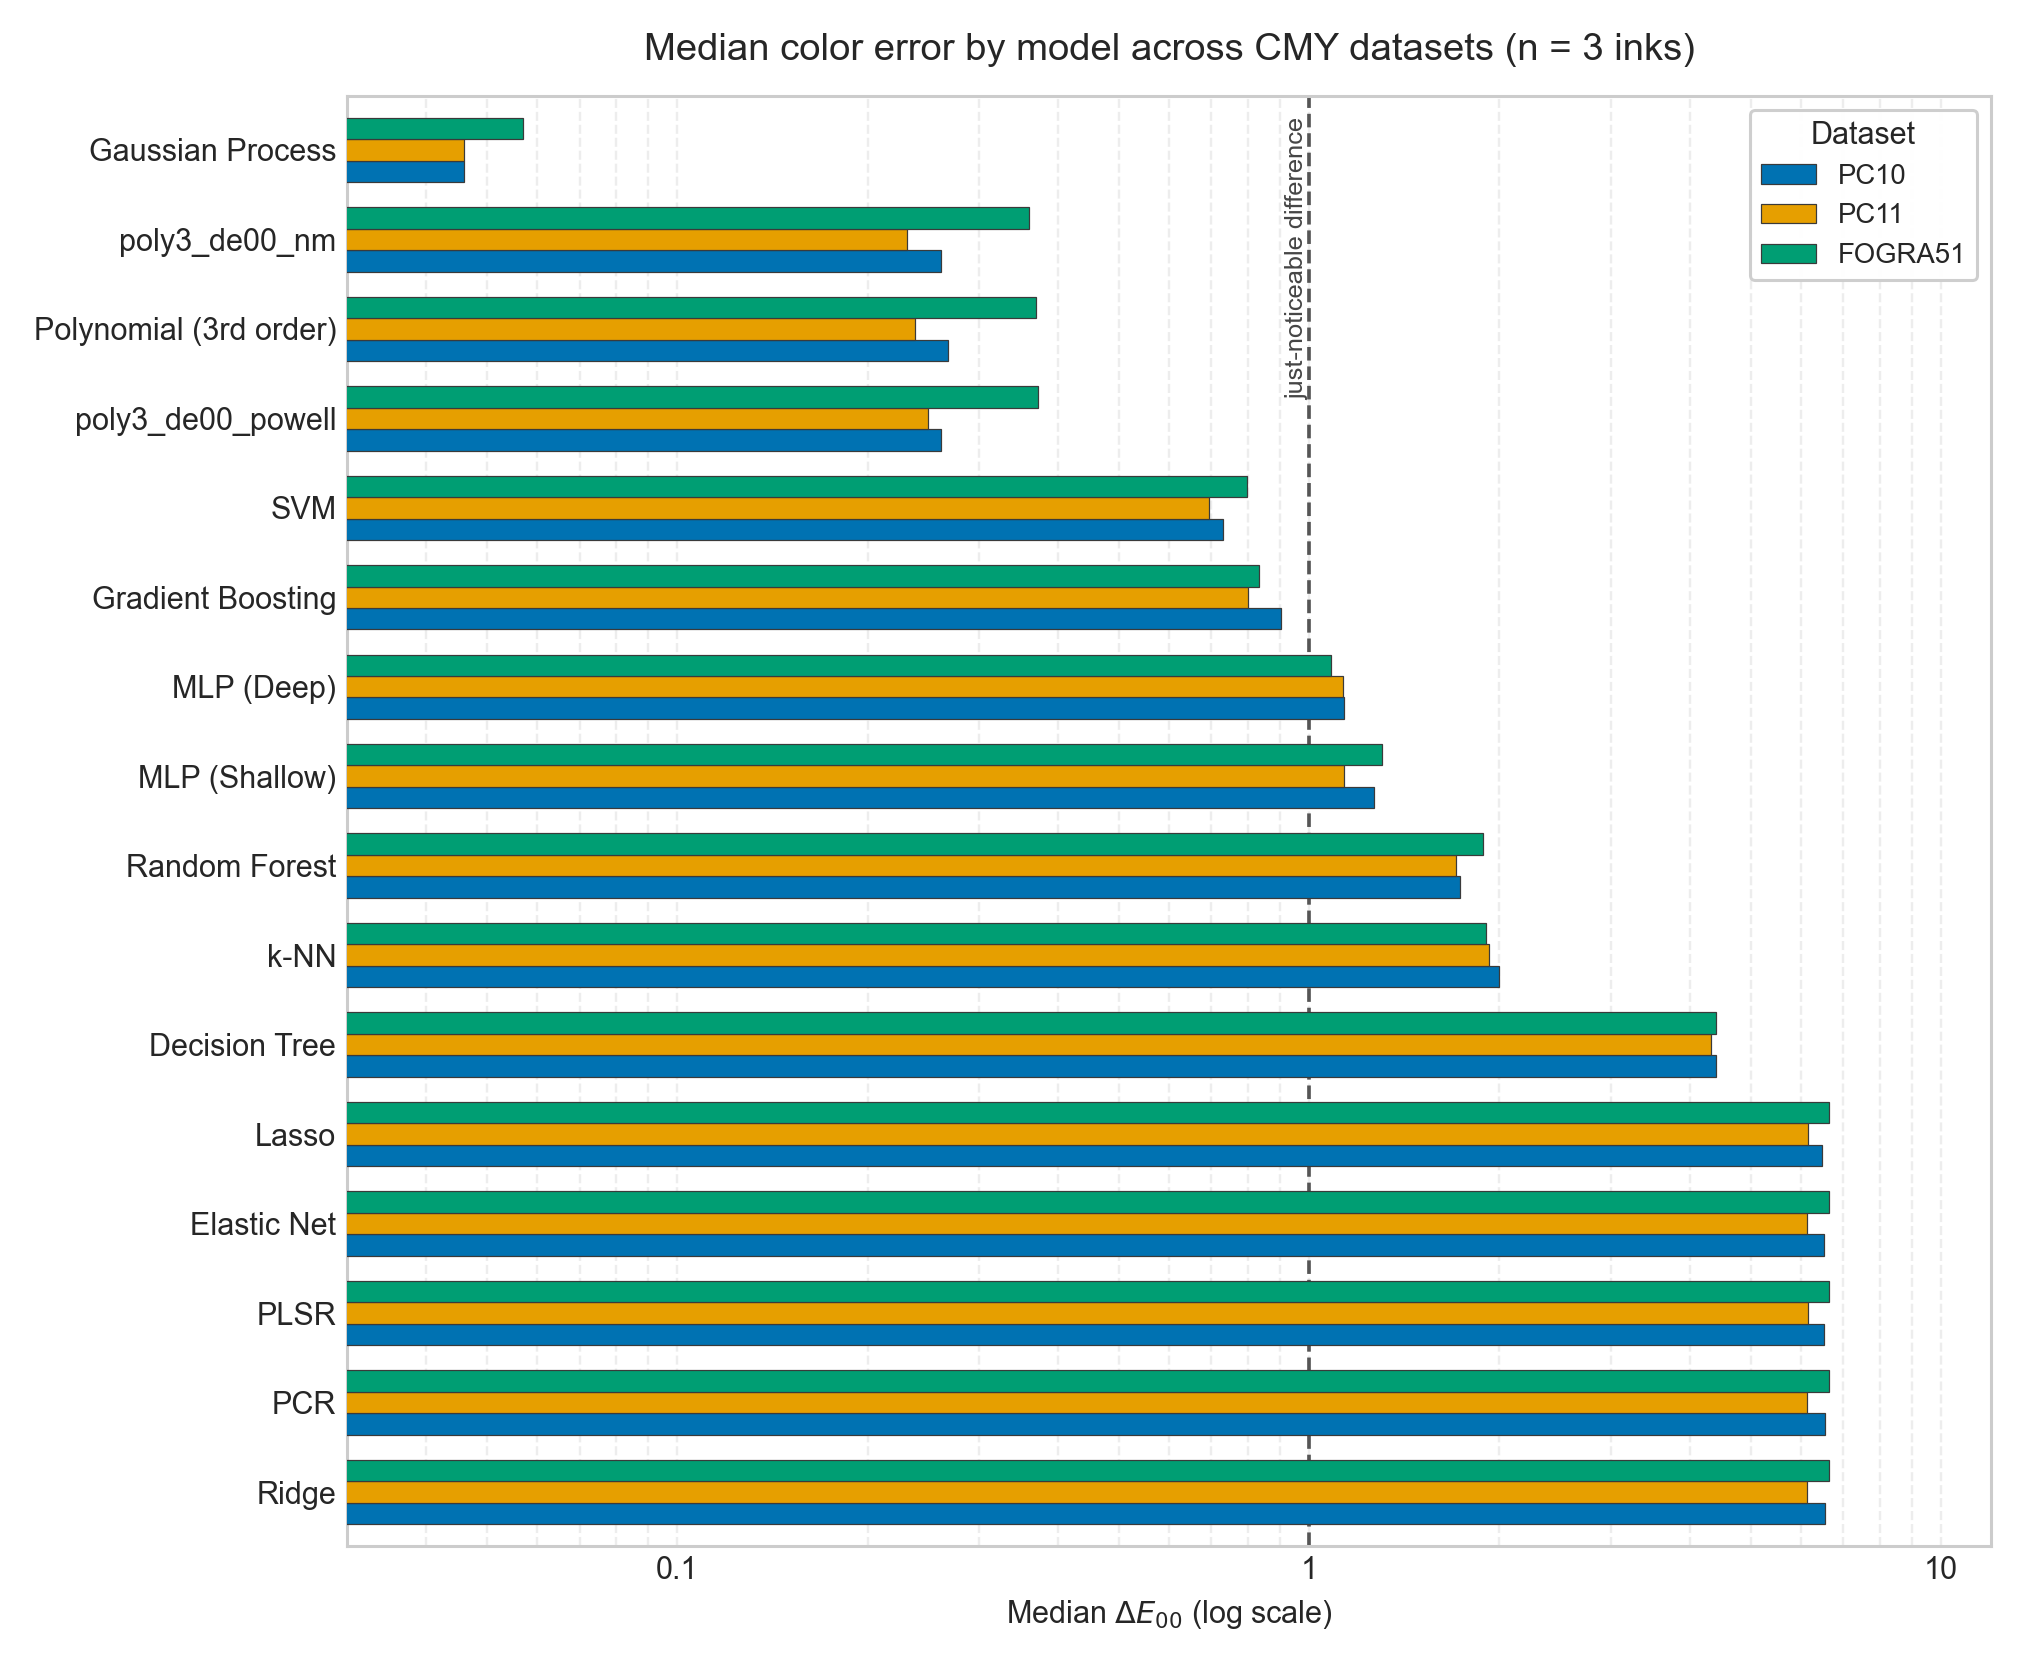
\includegraphics[width=0.85\textwidth]{../figures/fig_n3_model_comparison.png}
\caption{Median $\Delta E_{00}$ per model across the three CMY datasets
(818 $K=0$ samples each, 5-fold cross-validation), ranked by mean median
across datasets. Log scale; the dashed line marks the just-noticeable
difference ($\Delta E_{00} \approx 1$).}
\label{fig:n3comparison}
\end{figure}

\subsection{$n=4$ (CMYK) and the $n{=}3 \to n{=}4$ Comparison}
\respending{Table: median/P95/max $\Delta E_{00}$ per model per dataset
(*-CMYK). Source: \texttt{journal/results/\{PC10,PC11,FOGRA51\}-CMYK/summary.csv}.}

Figure~\ref{fig:n3vsn4} compares median $\Delta E_{00}$ at $n=3$ (CMY) versus
$n=4$ (CMYK) for every model on PC10, the full 1{,}617-sample set now
including the $K>0$ rows. Adding the fourth input channel is not uniformly
costly: third-order polynomial regression, which has no mechanism to
represent the extra channel's interaction terms beyond its fixed cubic
expansion, degrades from a median of 0.279 to 0.944 ($\times$3.4), whereas
Gaussian process regression is comparatively robust, degrading only from
0.054 to 0.063 ($\times$1.2). This asymmetry is consistent with GP
regression's non-parametric kernel adapting to the additional input
dimension, while the fixed-order polynomial basis cannot.

\begin{figure}[h]
\centering
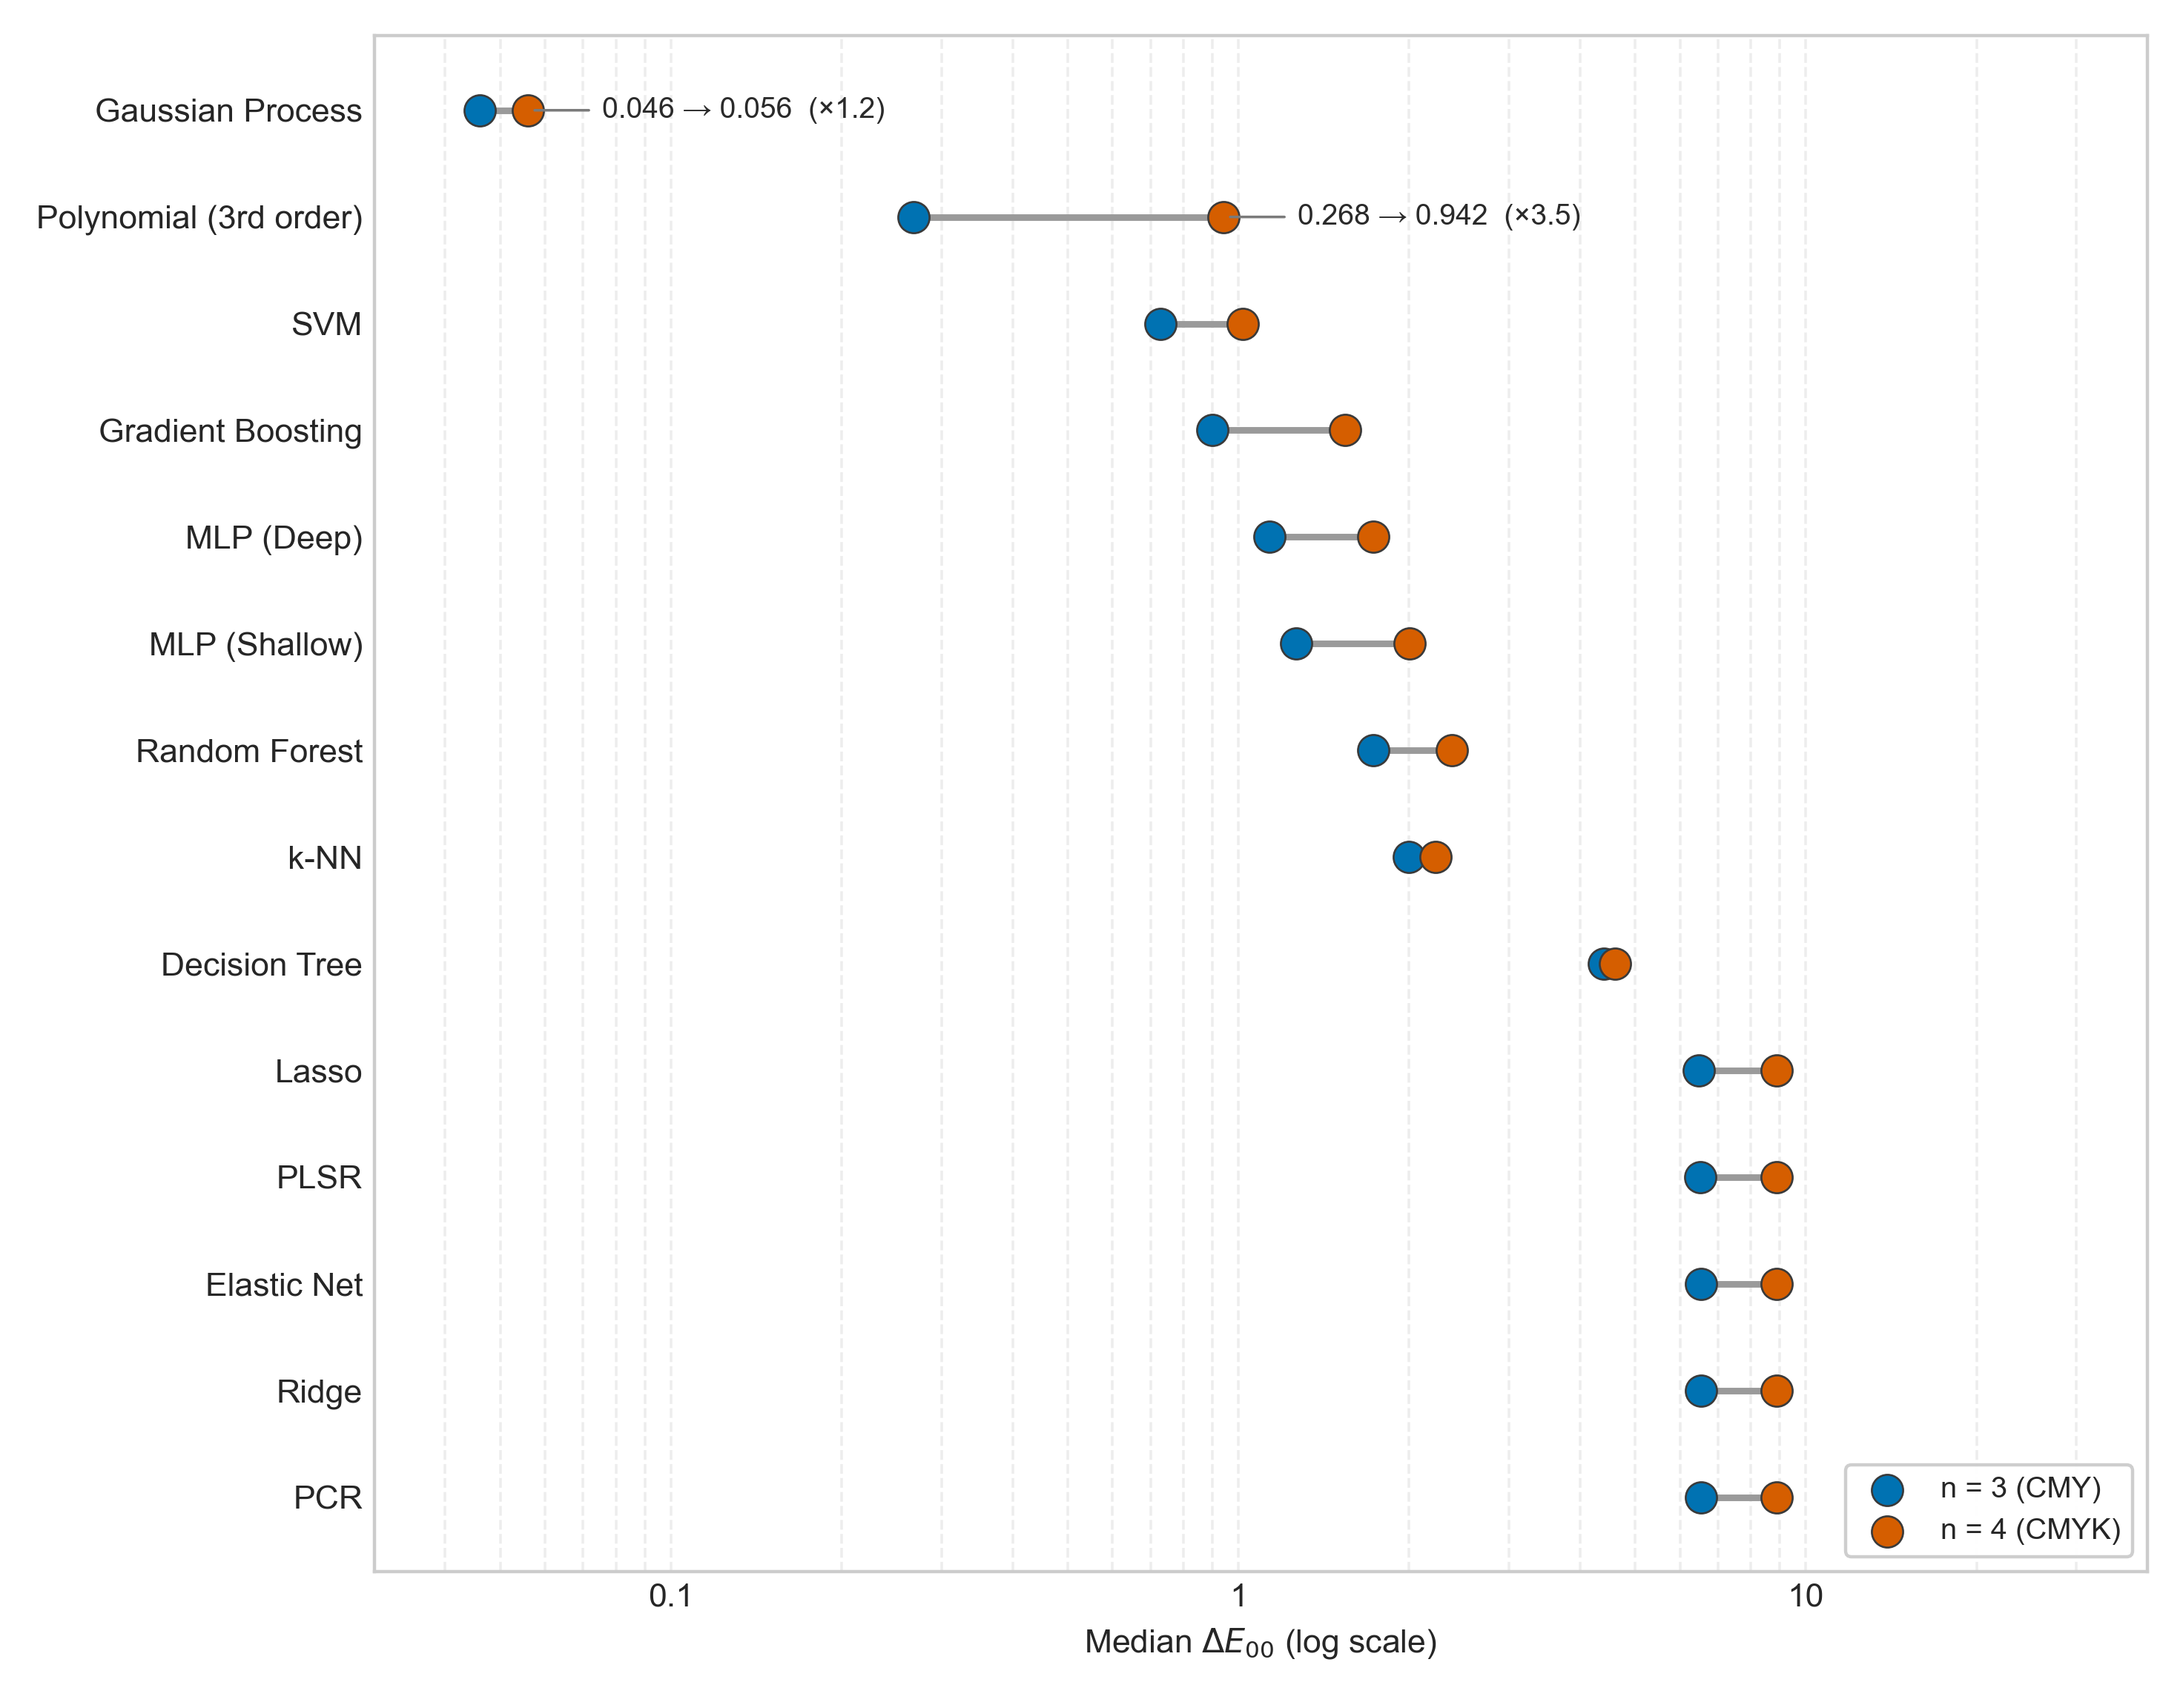
\includegraphics[width=0.85\textwidth]{../figures/fig_n3_vs_n4.png}
\caption{Median $\Delta E_{00}$ per model on PC10 at $n=3$ (CMY, 818 samples)
versus $n=4$ (CMYK, 1{,}617 samples). Polynomial regression degrades
$\times$3.4 with the added K channel, while Gaussian process regression
degrades only $\times$1.2, the two highlighted comparisons.}
\label{fig:n3vsn4}
\end{figure}

\subsection{Gaussian Process vs.\ Noise Floor}

Gaussian process regression is the best-median model in every
dataset/condition combination reported above. Because GP is also the model
most exposed to a subtle cross-validation leak -- duplicate colorant-input
rows with distinct measured XYZ landing in both the train and test folds --
its result was re-verified with a duplicate-grouped cross-validation split
(folds assigned by distinct input recipe rather than by row, so all
duplicates of a given recipe fall in the same fold; see
Section~\ref{sec:protocol}). Across all six dataset/condition combinations,
GP's median $\Delta E_{00}$ ranges from 0.052 to 0.073, and the
grouped-CV median never differs from the plain $k$-fold median by more than
a factor of 1.02, confirming the result is not an artifact of duplicate
leakage. Third-order polynomial regression, re-checked the same way, is
similarly stable. Source: \texttt{journal/results/gp\_verification.csv}.

\subsection{IFRA Newsprint: Within-Run, Cross-Run, and Leave-One-Out}
\respending{Plan 03 results, conditional on ingestion completing. Source:
\texttt{journal/results/ifra/*.csv}. Figure F4.}

\subsection{Direct $\Delta E_{00}$ Loss}
\respending{Plan 05 results, conditional on landing in time.}

\subsection{LLM-as-Color-Predictor}
\respending{Plan 04 results, conditional on landing in time. Source:
\texttt{journal/results/llm/comparison.csv}. Figure F5.}

\subsection{$n=7$ (CMYKOGV)}
\respending{Plan 06 results, conditional on the dataset arriving from Phil
in time. Figure F6 (median $\Delta E_{00}$ vs.\ $n \in \{3,4,7\}$).}

% =============================================================================
\section{Discussion}
% =============================================================================
\todonote{Task 2. Answer Phil's two core questions explicitly: (a) does any
ML method beat classical polynomial regression at $n \leq 4$, and if so by
how much, avoiding gray-component-replacement-style handling of K; (b) does
any method handle $n>4$ successfully where polynomial regression is not
designed to scale (contingent on the $n=7$ dataset). Limitations to cover:
single-substrate training sets (no cross-printer generalization claim
without the IFRA results); GP's $O(N^3)$ training-set-size scaling as a
practical deployment concern; the K-ambiguity lesson from the AIC 2025
conference version as a cautionary methodological note (kept minimal, per
author decision -- see Methods correction paragraph -- no separate pitfalls
section unless Phil asks for one on review).}

% =============================================================================
\section{Conclusion}
% =============================================================================
\todonote{Task 2. One paragraph, restating the corrected headline findings
and, if landed, the $n>4$ finding.}

% =============================================================================
\section*{Data Availability Statement}
% =============================================================================
Code and data supporting this study are available at
\url{https://github.com/hamzafer/Evaluating-Machine-Learning-Methods}.
\todonote{Confirm this is still the correct public repository URL before
submission (ported from the AIC 2025 conference paper's Code and Data
Availability section) and that it reflects the corrected pipeline described
here, not only the legacy AIC v1 code.}

% =============================================================================
% References
% =============================================================================
\bibliographystyle{unsrtnat}
% TODO: swap to MDPI's own .bst (in the Definitions/ subfolder of the
% official template) once downloaded; unsrtnat is a standard TeX Live style
% used here only so the document compiles standalone in the meantime.
\bibliography{refs}

\end{document}
